\documentclass{extbook}[14pt]
\usepackage{multicol, enumerate, enumitem, hyperref, color, soul, setspace, parskip, fancyhdr, amssymb, amsthm, amsmath, bbm, latexsym, units, mathtools}
\everymath{\displaystyle}
\usepackage[headsep=0.5cm,headheight=0cm, left=1 in,right= 1 in,top= 1 in,bottom= 1 in]{geometry}
\usepackage{dashrule}  % Package to use the command below to create lines between items
\newcommand{\litem}[1]{\item #1

\rule{\textwidth}{0.4pt}}
\pagestyle{fancy}
\lhead{}
\chead{Answer Key for Progress Quiz 5 Version A}
\rhead{}
\lfoot{9912-2038}
\cfoot{}
\rfoot{Spring 2021}
\begin{document}
\textbf{This key should allow you to understand why you choose the option you did (beyond just getting a question right or wrong). \href{https://xronos.clas.ufl.edu/mac1105spring2020/courseDescriptionAndMisc/Exams/LearningFromResults}{More instructions on how to use this key can be found here}.}

\textbf{If you have a suggestion to make the keys better, \href{https://forms.gle/CZkbZmPbC9XALEE88}{please fill out the short survey here}.}

\textit{Note: This key is auto-generated and may contain issues and/or errors. The keys are reviewed after each exam to ensure grading is done accurately. If there are issues (like duplicate options), they are noted in the offline gradebook. The keys are a work-in-progress to give students as many resources to improve as possible.}

\rule{\textwidth}{0.4pt}

\begin{enumerate}\litem{
Construct the lowest-degree polynomial given the zeros below. Then, choose the intervals that contain the coefficients of the polynomial in the form $ax^3+bx^2+cx+d$.
\[ \frac{5}{4}, \frac{-1}{4}, \text{ and } \frac{-5}{2} \]The solution is \( 32x^{3} +48 x^{2} -90 x -25 \), which is option B.\begin{enumerate}[label=\Alph*.]
\item \( a \in [31, 39], b \in [125, 129], c \in [125, 134], \text{ and } d \in [25, 29] \)

$32x^{3} +128 x^{2} +130 x + 25$, which corresponds to multiplying out $(4x + 5)(4x + 1)(2x + 5)$.
\item \( a \in [31, 39], b \in [44, 51], c \in [-91, -83], \text{ and } d \in [-30, -22] \)

* $32x^{3} +48 x^{2} -90 x -25$, which is the correct option.
\item \( a \in [31, 39], b \in [-57, -45], c \in [-91, -83], \text{ and } d \in [25, 29] \)

$32x^{3} -48 x^{2} -90 x + 25$, which corresponds to multiplying out $(4x + 5)(4x -1)(2x -5)$.
\item \( a \in [31, 39], b \in [111, 113], c \in [70, 76], \text{ and } d \in [-30, -22] \)

$32x^{3} +112 x^{2} +70 x -25$, which corresponds to multiplying out $(4x + 5)(4x -1)(2x + 5)$.
\item \( a \in [31, 39], b \in [44, 51], c \in [-91, -83], \text{ and } d \in [25, 29] \)

$32x^{3} +48 x^{2} -90 x + 25$, which corresponds to multiplying everything correctly except the constant term.
\end{enumerate}

\textbf{General Comment:} To construct the lowest-degree polynomial, you want to multiply out $(4x -5)(4x + 1)(2x + 5)$
}
\litem{
Describe the zero behavior of the zero $x = -3$ of the polynomial below.
\[ f(x) = 8(x + 3)^{3}(x - 3)^{4}(x + 8)^{2}(x - 8)^{3} \]The solution is the graph below, which is option A.
\begin{center}
    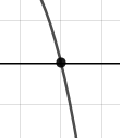
\includegraphics[width=0.3\textwidth]{../Figures/polyZeroBehaviorAA.png}
\end{center}\begin{enumerate}[label=\Alph*.]
\begin{multicols}{2}
\item 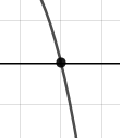
\includegraphics[width = 0.3\textwidth]{../Figures/polyZeroBehaviorAA.png}
\item 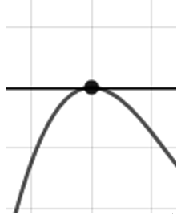
\includegraphics[width = 0.3\textwidth]{../Figures/polyZeroBehaviorBA.png}
\item 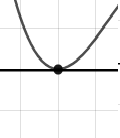
\includegraphics[width = 0.3\textwidth]{../Figures/polyZeroBehaviorCA.png}
\item 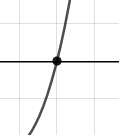
\includegraphics[width = 0.3\textwidth]{../Figures/polyZeroBehaviorDA.png}
\end{multicols}\item None of the above.\end{enumerate}
\textbf{General Comment:} You will need to sketch the entire graph, then zoom in on the zero the question asks about.
}
\litem{
Describe the end behavior of the polynomial below.
\[ f(x) = -4(x - 9)^{3}(x + 9)^{8}(x + 3)^{5}(x - 3)^{7} \]The solution is the graph below, which is option A.
\begin{center}
    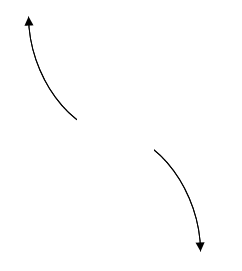
\includegraphics[width=0.3\textwidth]{../Figures/polyEndBehaviorAA.png}
\end{center}\begin{enumerate}[label=\Alph*.]
\begin{multicols}{2}
\item 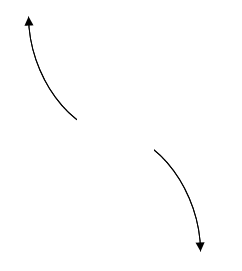
\includegraphics[width = 0.3\textwidth]{../Figures/polyEndBehaviorAA.png}
\item 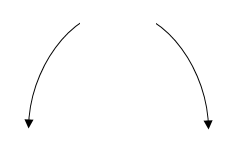
\includegraphics[width = 0.3\textwidth]{../Figures/polyEndBehaviorBA.png}
\item 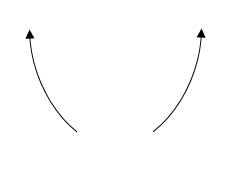
\includegraphics[width = 0.3\textwidth]{../Figures/polyEndBehaviorCA.png}
\item 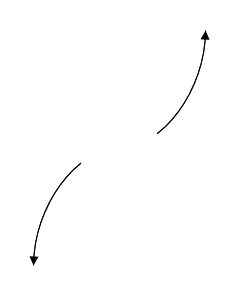
\includegraphics[width = 0.3\textwidth]{../Figures/polyEndBehaviorDA.png}
\end{multicols}\item None of the above.\end{enumerate}
\textbf{General Comment:} Remember that end behavior is determined by the leading coefficient AND whether the \textbf{sum} of the multiplicities is positive or negative.
}
\litem{
Describe the zero behavior of the zero $x = -3$ of the polynomial below.
\[ f(x) = 7(x + 2)^{8}(x - 2)^{7}(x - 3)^{11}(x + 3)^{8} \]The solution is the graph below, which is option C.
\begin{center}
    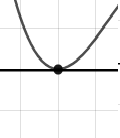
\includegraphics[width=0.3\textwidth]{../Figures/polyZeroBehaviorCopyCA.png}
\end{center}\begin{enumerate}[label=\Alph*.]
\begin{multicols}{2}
\item 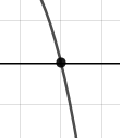
\includegraphics[width = 0.3\textwidth]{../Figures/polyZeroBehaviorCopyAA.png}
\item 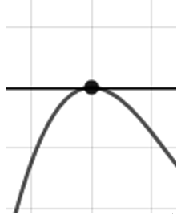
\includegraphics[width = 0.3\textwidth]{../Figures/polyZeroBehaviorCopyBA.png}
\item 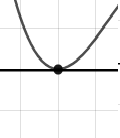
\includegraphics[width = 0.3\textwidth]{../Figures/polyZeroBehaviorCopyCA.png}
\item 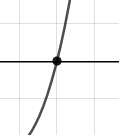
\includegraphics[width = 0.3\textwidth]{../Figures/polyZeroBehaviorCopyDA.png}
\end{multicols}\item None of the above.\end{enumerate}
\textbf{General Comment:} You will need to sketch the entire graph, then zoom in on the zero the question asks about.
}
\litem{
Describe the end behavior of the polynomial below.
\[ f(x) = 4(x + 6)^{2}(x - 6)^{7}(x - 8)^{5}(x + 8)^{7} \]The solution is the graph below, which is option D.
\begin{center}
    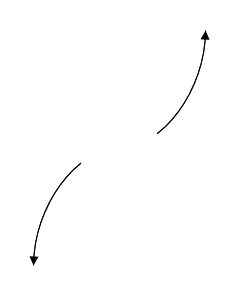
\includegraphics[width=0.3\textwidth]{../Figures/polyEndBehaviorCopyDA.png}
\end{center}\begin{enumerate}[label=\Alph*.]
\begin{multicols}{2}
\item 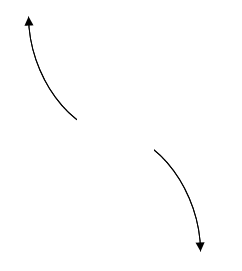
\includegraphics[width = 0.3\textwidth]{../Figures/polyEndBehaviorCopyAA.png}
\item 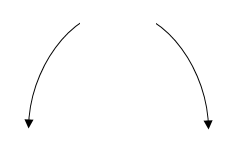
\includegraphics[width = 0.3\textwidth]{../Figures/polyEndBehaviorCopyBA.png}
\item 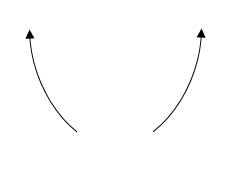
\includegraphics[width = 0.3\textwidth]{../Figures/polyEndBehaviorCopyCA.png}
\item 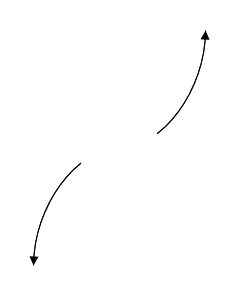
\includegraphics[width = 0.3\textwidth]{../Figures/polyEndBehaviorCopyDA.png}
\end{multicols}\item None of the above.\end{enumerate}
\textbf{General Comment:} Remember that end behavior is determined by the leading coefficient AND whether the \textbf{sum} of the multiplicities is positive or negative.
}
\litem{
Construct the lowest-degree polynomial given the zeros below. Then, choose the intervals that contain the coefficients of the polynomial in the form $x^3+bx^2+cx+d$.
\[ -3 + 2 i \text{ and } 4 \]The solution is \( x^{3} +2 x^{2} -11 x -52 \), which is option A.\begin{enumerate}[label=\Alph*.]
\item \( b \in [1.3, 4.5], c \in [-12.6, -8.5], \text{ and } d \in [-54, -46] \)

* $x^{3} +2 x^{2} -11 x -52$, which is the correct option.
\item \( b \in [-0.4, 1.2], c \in [-6.2, -5.7], \text{ and } d \in [-1, 10] \)

$x^{3} + x^{2} -6 x + 8$, which corresponds to multiplying out $(x -2)(x -4)$.
\item \( b \in [-0.4, 1.2], c \in [-2.3, -0.7], \text{ and } d \in [-14, -8] \)

$x^{3} + x^{2} -x -12$, which corresponds to multiplying out $(x + 3)(x -4)$.
\item \( b \in [-2.6, -1.3], c \in [-12.6, -8.5], \text{ and } d \in [48, 58] \)

$x^{3} -2 x^{2} -11 x + 52$, which corresponds to multiplying out $(x-(-3 + 2 i))(x-(-3 - 2 i))(x + 4)$.
\item \( \text{None of the above.} \)

This corresponds to making an unanticipated error or not understanding how to use nonreal complex numbers to create the lowest-degree polynomial. If you chose this and are not sure what you did wrong, please contact the coordinator for help.
\end{enumerate}

\textbf{General Comment:} Remember that the conjugate of $a+bi$ is $a-bi$. Since these zeros always come in pairs, we need to multiply out $(x-(-3 + 2 i))(x-(-3 - 2 i))(x-(4))$.
}
\litem{
Construct the lowest-degree polynomial given the zeros below. Then, choose the intervals that contain the coefficients of the polynomial in the form $x^3+bx^2+cx+d$.
\[ -4 + 2 i \text{ and } 1 \]The solution is \( x^{3} +7 x^{2} +12 x -20 \), which is option D.\begin{enumerate}[label=\Alph*.]
\item \( b \in [-1, 5], c \in [3, 4], \text{ and } d \in [-6, -3] \)

$x^{3} + x^{2} +3 x -4$, which corresponds to multiplying out $(x + 4)(x -1)$.
\item \( b \in [-12, -5], c \in [6, 24], \text{ and } d \in [20, 27] \)

$x^{3} -7 x^{2} +12 x + 20$, which corresponds to multiplying out $(x-(-4 + 2 i))(x-(-4 - 2 i))(x + 1)$.
\item \( b \in [-1, 5], c \in [-3, 1], \text{ and } d \in [1, 6] \)

$x^{3} + x^{2} -3 x + 2$, which corresponds to multiplying out $(x -2)(x -1)$.
\item \( b \in [5, 11], c \in [6, 24], \text{ and } d \in [-23, -18] \)

* $x^{3} +7 x^{2} +12 x -20$, which is the correct option.
\item \( \text{None of the above.} \)

This corresponds to making an unanticipated error or not understanding how to use nonreal complex numbers to create the lowest-degree polynomial. If you chose this and are not sure what you did wrong, please contact the coordinator for help.
\end{enumerate}

\textbf{General Comment:} Remember that the conjugate of $a+bi$ is $a-bi$. Since these zeros always come in pairs, we need to multiply out $(x-(-4 + 2 i))(x-(-4 - 2 i))(x-(1))$.
}
\litem{
Which of the following equations \textit{could} be of the graph presented below?

\begin{center}
    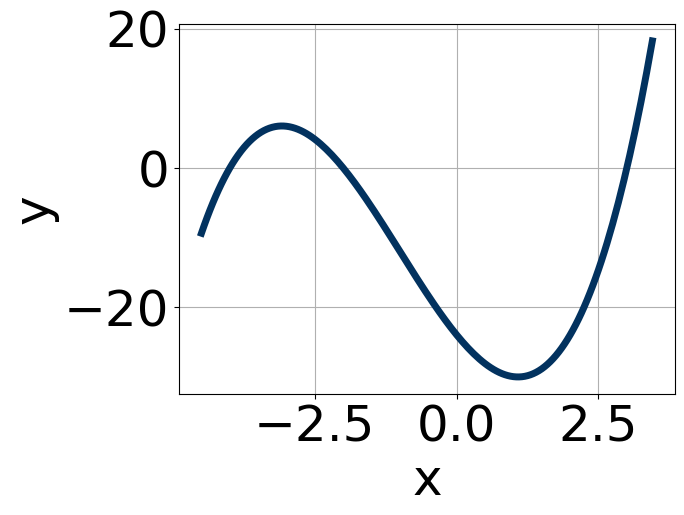
\includegraphics[width=0.5\textwidth]{../Figures/polyGraphToFunctionCopyA.png}
\end{center}


The solution is \( 8(x - 3)^{4} (x - 2)^{5} (x + 1)^{5} \), which is option E.\begin{enumerate}[label=\Alph*.]
\item \( -14(x - 3)^{6} (x - 2)^{11} (x + 1)^{10} \)

The factor $(x + 1)$ should have an odd power and the leading coefficient should be the opposite sign.
\item \( 7(x - 3)^{9} (x - 2)^{6} (x + 1)^{11} \)

The factor $3$ should have an even power and the factor $2$ should have an odd power.
\item \( -7(x - 3)^{8} (x - 2)^{7} (x + 1)^{9} \)

This corresponds to the leading coefficient being the opposite value than it should be.
\item \( 9(x - 3)^{6} (x - 2)^{4} (x + 1)^{11} \)

The factor $(x - 2)$ should have an odd power.
\item \( 8(x - 3)^{4} (x - 2)^{5} (x + 1)^{5} \)

* This is the correct option.
\end{enumerate}

\textbf{General Comment:} General Comments: Draw the x-axis to determine which zeros are touching (and so have even multiplicity) or cross (and have odd multiplicity).
}
\litem{
Construct the lowest-degree polynomial given the zeros below. Then, choose the intervals that contain the coefficients of the polynomial in the form $ax^3+bx^2+cx+d$.
\[ -1, \frac{-1}{2}, \text{ and } \frac{4}{3} \]The solution is \( 6x^{3} + x^{2} -9 x -4 \), which is option A.\begin{enumerate}[label=\Alph*.]
\item \( a \in [4, 11], b \in [-0.8, 1.7], c \in [-20, -8], \text{ and } d \in [-6, -2] \)

* $6x^{3} + x^{2} -9 x -4$, which is the correct option.
\item \( a \in [4, 11], b \in [-0.8, 1.7], c \in [-20, -8], \text{ and } d \in [3, 5] \)

$6x^{3} + x^{2} -9 x + 4$, which corresponds to multiplying everything correctly except the constant term.
\item \( a \in [4, 11], b \in [-3, -0.3], c \in [-20, -8], \text{ and } d \in [3, 5] \)

$6x^{3} -1 x^{2} -9 x + 4$, which corresponds to multiplying out $(x -1)(2x -1)(3x + 4)$.
\item \( a \in [4, 11], b \in [-18.5, -15.8], c \in [12, 20], \text{ and } d \in [-6, -2] \)

$6x^{3} -17 x^{2} +15 x -4$, which corresponds to multiplying out $(x -1)(2x -1)(3x -4)$.
\item \( a \in [4, 11], b \in [-12.4, -10.2], c \in [-2, 7], \text{ and } d \in [3, 5] \)

$6x^{3} -11 x^{2} +x + 4$, which corresponds to multiplying out $(x -1)(2x + 1)(3x -4)$.
\end{enumerate}

\textbf{General Comment:} To construct the lowest-degree polynomial, you want to multiply out $(x + 1)(2x + 1)(3x -4)$
}
\litem{
Which of the following equations \textit{could} be of the graph presented below?

\begin{center}
    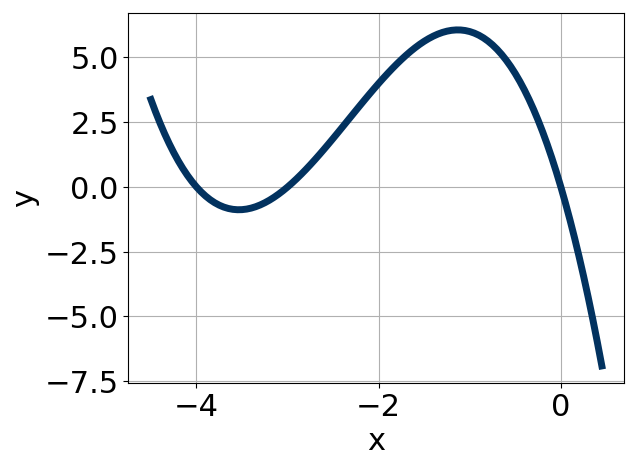
\includegraphics[width=0.5\textwidth]{../Figures/polyGraphToFunctionA.png}
\end{center}


The solution is \( 20(x + 1)^{4} (x + 2)^{9} (x - 3)^{11} \), which is option B.\begin{enumerate}[label=\Alph*.]
\item \( -20(x + 1)^{8} (x + 2)^{9} (x - 3)^{11} \)

This corresponds to the leading coefficient being the opposite value than it should be.
\item \( 20(x + 1)^{4} (x + 2)^{9} (x - 3)^{11} \)

* This is the correct option.
\item \( 11(x + 1)^{9} (x + 2)^{10} (x - 3)^{9} \)

The factor $-1$ should have an even power and the factor $-2$ should have an odd power.
\item \( -3(x + 1)^{10} (x + 2)^{5} (x - 3)^{4} \)

The factor $(x - 3)$ should have an odd power and the leading coefficient should be the opposite sign.
\item \( 4(x + 1)^{4} (x + 2)^{10} (x - 3)^{5} \)

The factor $(x + 2)$ should have an odd power.
\end{enumerate}

\textbf{General Comment:} General Comments: Draw the x-axis to determine which zeros are touching (and so have even multiplicity) or cross (and have odd multiplicity).
}
\end{enumerate}

\end{document}